\documentclass[a4paper,12pt]{article}

\usepackage[T2A]{fontenc}			
\usepackage[utf8]{inputenc}			
\usepackage[english,russian]{babel}	

\usepackage[
bookmarks=true, colorlinks=true, unicode=true,
urlcolor=black,linkcolor=black, anchorcolor=black,
citecolor=black, menucolor=black, filecolor=black,
]{hyperref}

\usepackage{color}
\usepackage{caption}
\DeclareCaptionFont{white}{\color{black}}
\DeclareCaptionFormat{listing}{\colorbox{white}{\parbox{\textwidth}{#1#2#3}}}
\captionsetup[lstlisting]{format=listing,labelfont=white,textfont=white}

\usepackage{amsmath,amsfonts,amssymb,amsthm,mathtools} 
\usepackage{wasysym}

\usepackage{graphicx}
%\usepackage[cache=false]{minted}
\usepackage{cmap}
\usepackage{indentfirst}

\usepackage{listings} 
\usepackage{fancyvrb}

\usepackage{geometry}
\geometry{left=2cm}
\geometry{right=1.5cm}
\geometry{top=1cm}
\geometry{bottom=2cm}

\setlength{\parindent}{5ex}
\setlength{\parskip}{0.5em}

\usepackage{pgfplots}
\usetikzlibrary{datavisualization}
\usetikzlibrary{datavisualization.formats.functions}

\begin{document}
	\lstset{ %
		language=C,                 % выбор языка для подсветки (здесь это С)
		basicstyle=\small\sffamily, % размер и начертание шрифта для подсветки кода
		numbers=left,               % где поставить нумерацию строк (слева\справа)
		numberstyle=\tiny,           % размер шрифта для номеров строк
		stepnumber=1,                   % размер шага между двумя номерами строк
		numbersep=5pt,                % как далеко отстоят номера строк от подсвечиваемого кода
		backgroundcolor=\color{white}, % цвет фона подсветки - используем \usepackage{color}
		showspaces=false,            % показывать или нет пробелы специальными отступами
		showstringspaces=false,      % показывать или нет пробелы в строках
		showtabs=false,             % показывать или нет табуляцию в строках
		frame=single,              % рисовать рамку вокруг кода
		tabsize=2,                 % размер табуляции по умолчанию равен 2 пробелам
		captionpos=t,              % позиция заголовка вверху [t] или внизу [b] 
		breaklines=true,           % автоматически переносить строки (да\нет)
		breakatwhitespace=false, % переносить строки только если есть пробел
		escapeinside={\%*}{*)}   % если нужно добавить комментарии в коде
	}
	
	% Титульный лист
	\begin{figure}[h!]
		\begin{center}
			{
\includegraphics[scale = 0.4]{titul.jpg}}
			\label{titul}
		\end{center}
	\end{figure}
	
	\vspace*{15mm} 
	
	\huge
	\begin{center}
		Дисциплина: <<Функциональное и логическое программирование>>
	\end{center}
	\vspace*{15mm} 	
	
	\begin{center}
		Лабораторная работа №11
	\end{center}
	
	\vspace*{15mm} 	
	
	\large
	\begin{flushright}
		Студент: Левушкин И. К. \\
		Группа: ИУ7-62Б \\
		Преподаватели: Толпинская Н. Б., \\ Строганов Ю. В. \\
	\end{flushright}
	
	\vspace*{30mm}
	\begin{center}
		Москва, 2020 г.  
	\end{center}
	\thispagestyle{empty}
	
	
	\newpage
	
	\section{Запуск среды Visual Prolog 5.2 и настройка утилиты TestGoal}
	
	Среда \textit{Visual Prolog 5.2} установлена, запущена и настроена утилита \textit{TestGoal} в соответствии с дополнительными материалами к 11 лабораторной работе.
	
	Установка была произведена на операционную систему \textit{Windows XP}, запущенную из-под виртуальной среды \textit{Parallels Desktop}.
	
	\begin{figure}[h!]
		\begin{center}
			{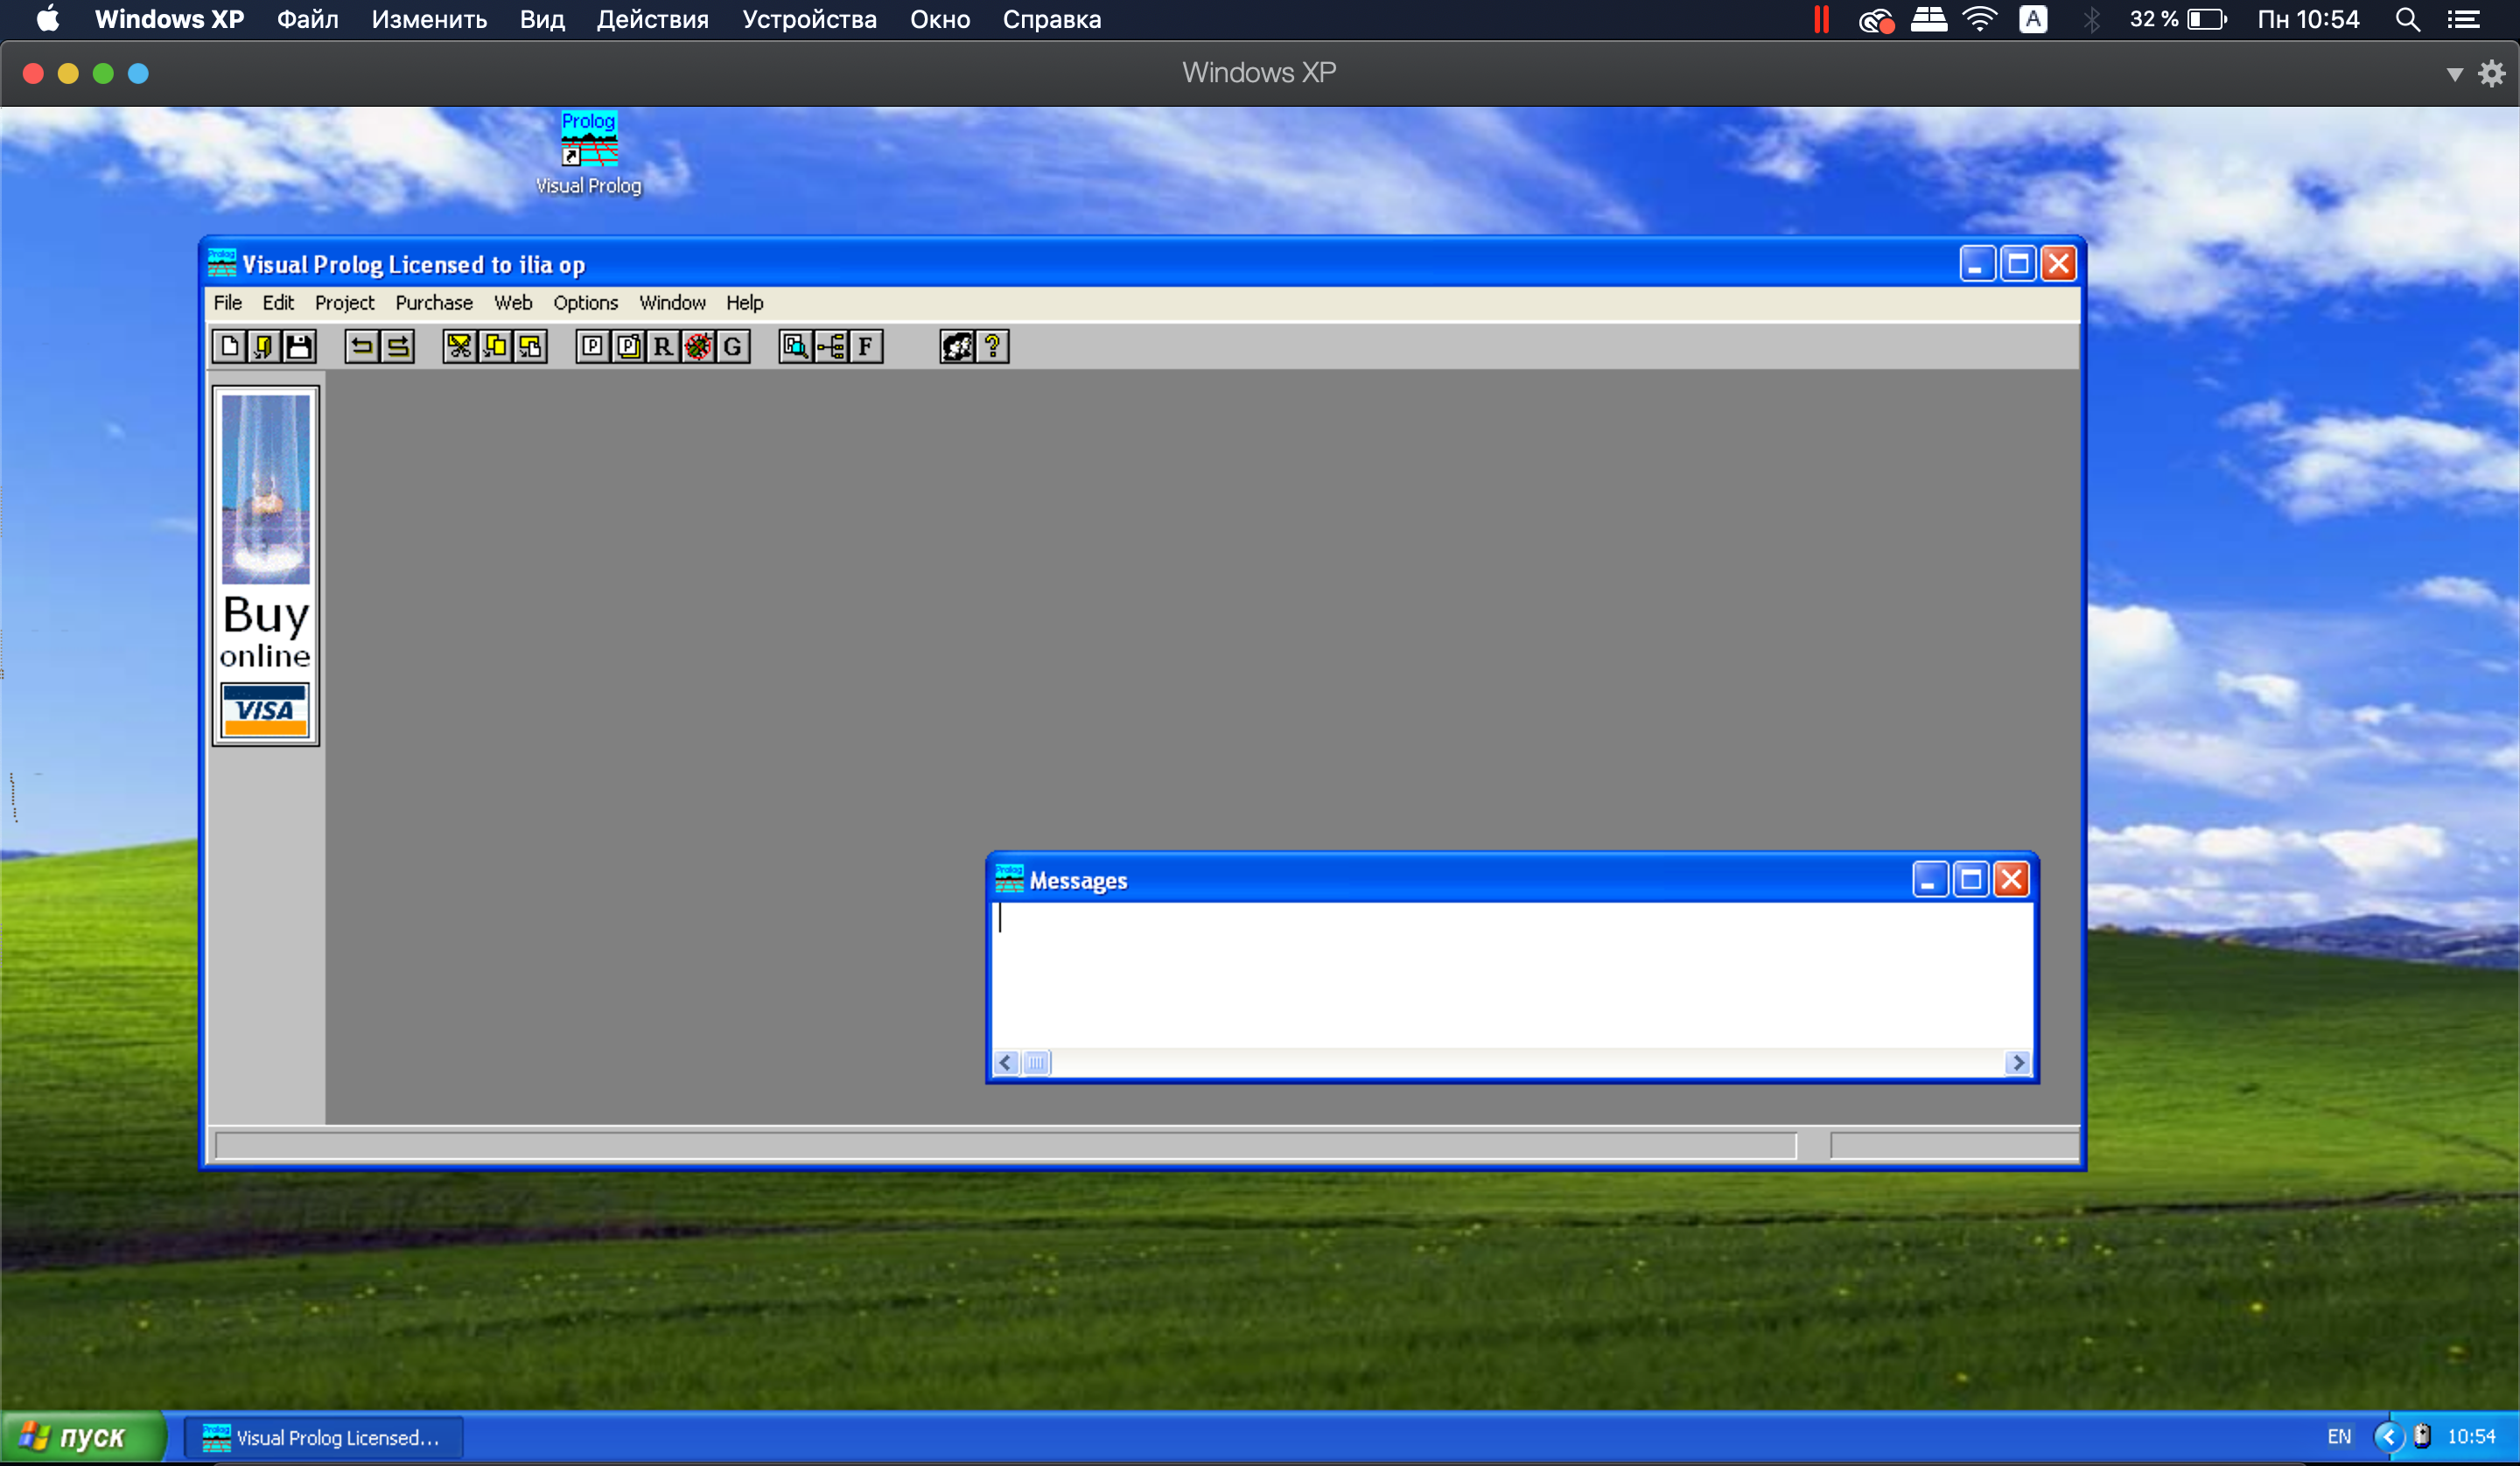
\includegraphics[scale = 0.3]{parallels.png}}
			\label{parallels}
		\end{center}
	\caption{Запуск среды \textit{Visual Prolog 5.2} на \textit{Windows XP} из-под \textit{Parallels Desktop}.}
	\end{figure}
	
	\newpage
	
	\section{Запуск тестовых программ}
	
	\subsection{Пример с выводом множества ответов}
	
	Следующая программа демонстрирует возможности утилиты \textit{TestGoal}, а именно:  поиск всех решений для определенной в программе цели. Для каждого
	решения \textit{TestGoal} отображает значения всех переменных из секции \textit{GOAL} и число решений.
	
		\begin{figure}[h!]
		\begin{center}
			\begin{minipage}[h!]{0.3\linewidth}
				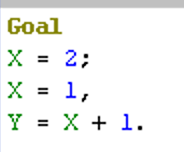
\includegraphics[width=1\linewidth]{goal.png}
			\end{minipage}
			\begin{minipage}[h!]{0.3\linewidth}
				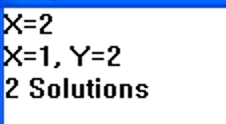
\includegraphics[width=1\linewidth]{result.png}
			\end{minipage}
			\label{ris:testgoal}
			\caption{Вывод режима \textit{TestGoal}.}
		\end{center}
	\end{figure}
	
	\subsection{Пример ch02e01.pro}
	
	Следующая программа создает предикат \textit{likes(symbol, symbol)}. И в разделе \textit{clauses} записывается 4 факта и 1 правило: Биллу нравится то же, что и tom: \textit{likes(bill, Activity):- likes(tom, Activity)}. В разделе goal на первом скриншоте задается вопрос: \textit{Bill likes baseball?}
	
	Поскольку Тому нравится baseball, ответ да:
	
	\begin{figure}[h!]
		\begin{center}
			{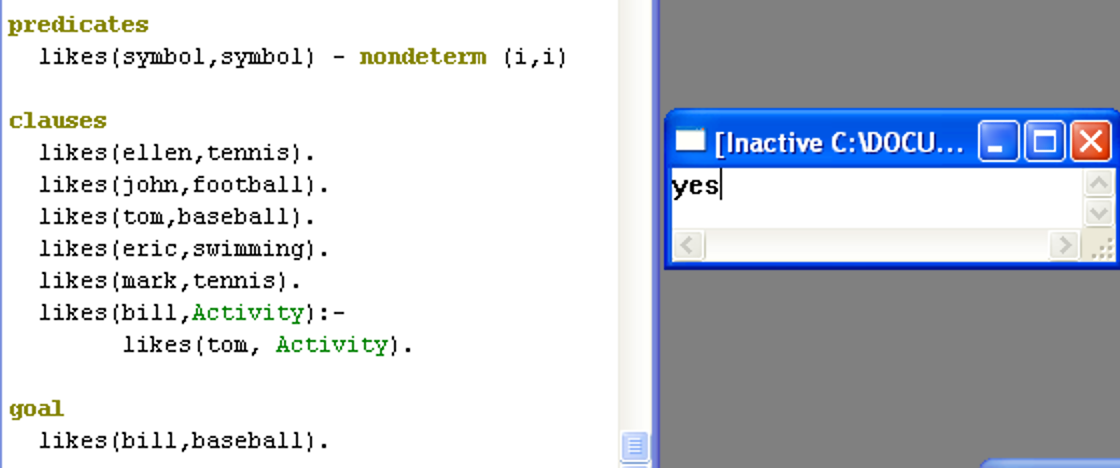
\includegraphics[scale = 0.7]{ch02e01_1.png}}
			\label{ch02e01_1}
		\end{center}
		\caption{Программа ch02e01\_1.pro.}
	\end{figure}

	\newpage

	В разделе goal на втором скриншоте задается вопрос: \textit{Bill likes tennis?}
	
	Поскольку ни Билл, ни Том не увлекаются теннисом, ответ нет:
	
	\begin{figure}[h!]
		\begin{center}
			{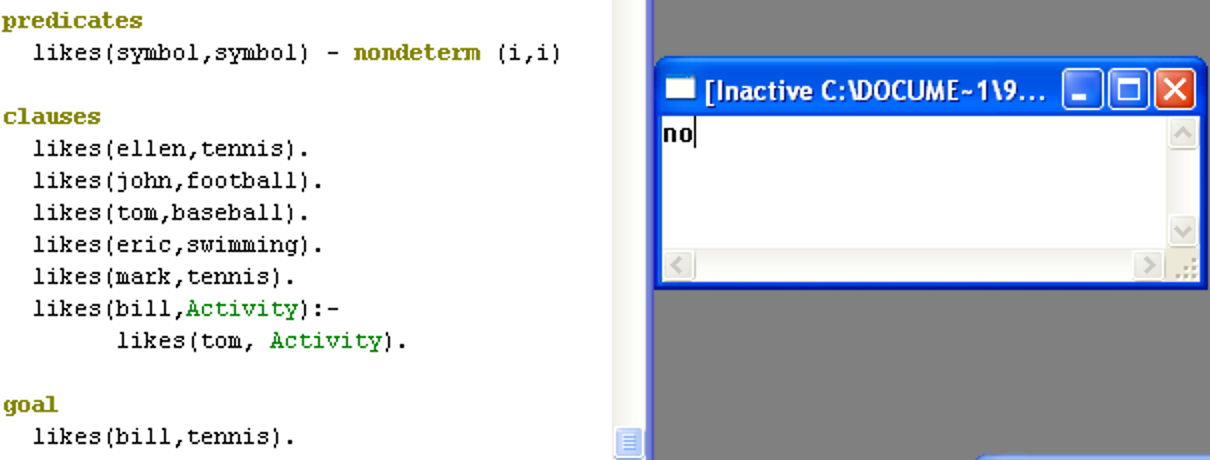
\includegraphics[scale = 0.7]{ch02e01_2.png}}
			\label{ch02e01_2}
		\end{center}
		\caption{Программа ch02e01\_2.pro.}
	\end{figure}
	
	\section{Программа Телефонный справочник}
	
	Ниже приведена программа телефонный справочник, использующая только один предикат: \textit{phone\_list(string First, string Last, string Phone, string Month, integer Day, integer Year)}:
	
	\begin{figure}[h!]
		\begin{center}
			{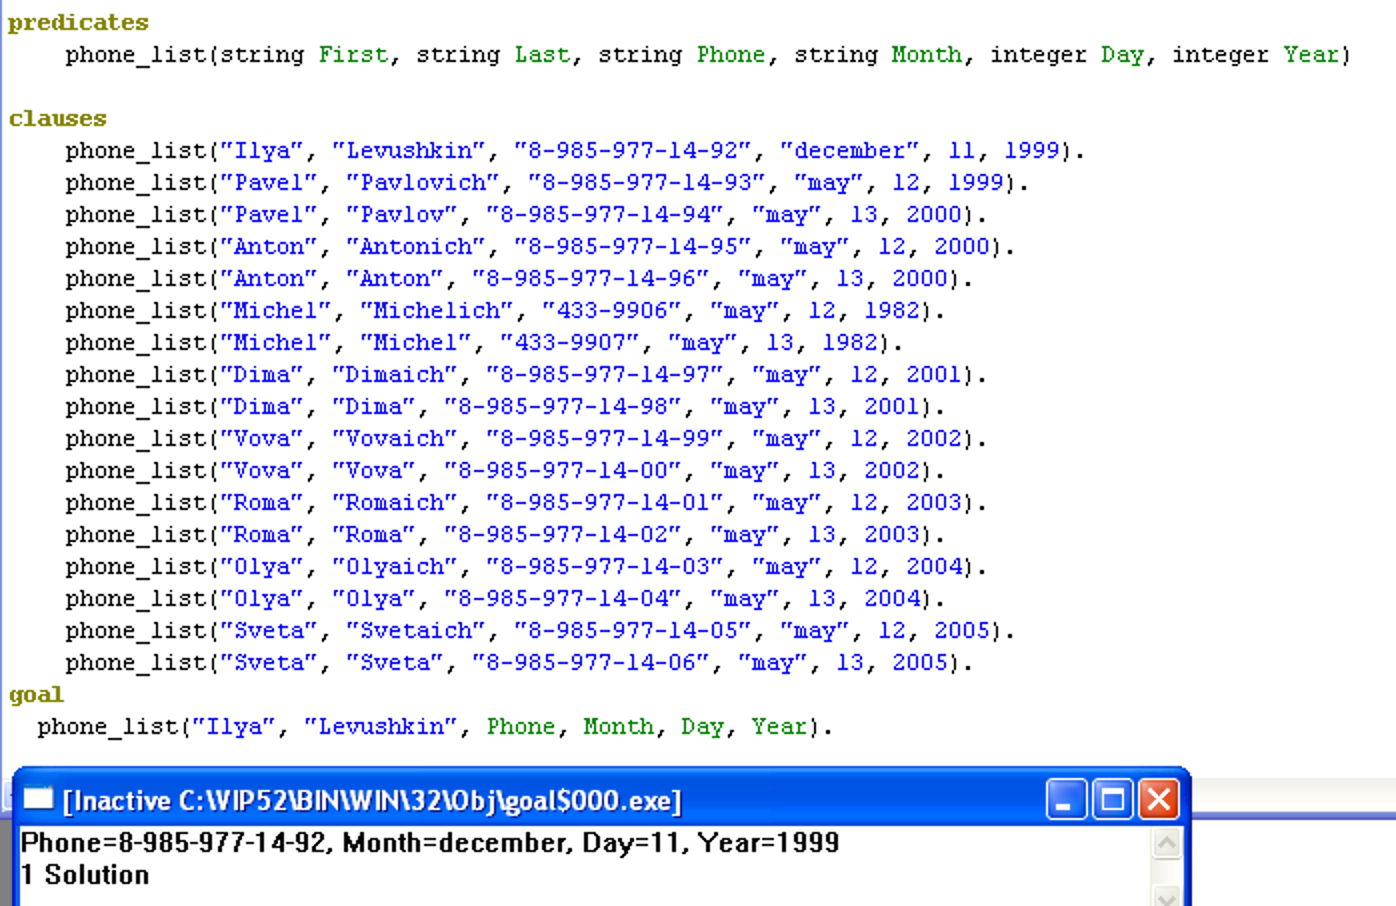
\includegraphics[scale = 0.7]{program_1.png}}
			\label{prog_1}
		\end{center}
		\caption{Программа Test.pro.}
	\end{figure}

	\newpage

	В разделе goal задается вопрос: Есть ли \textit{Ilya Levushkin} в телефонной книге?
	
	Ответ будет содержать всех таких \textit{Ilya Levushkin} (в данном случае одного).
	
	\begin{figure}[h!]
		\begin{center}
			{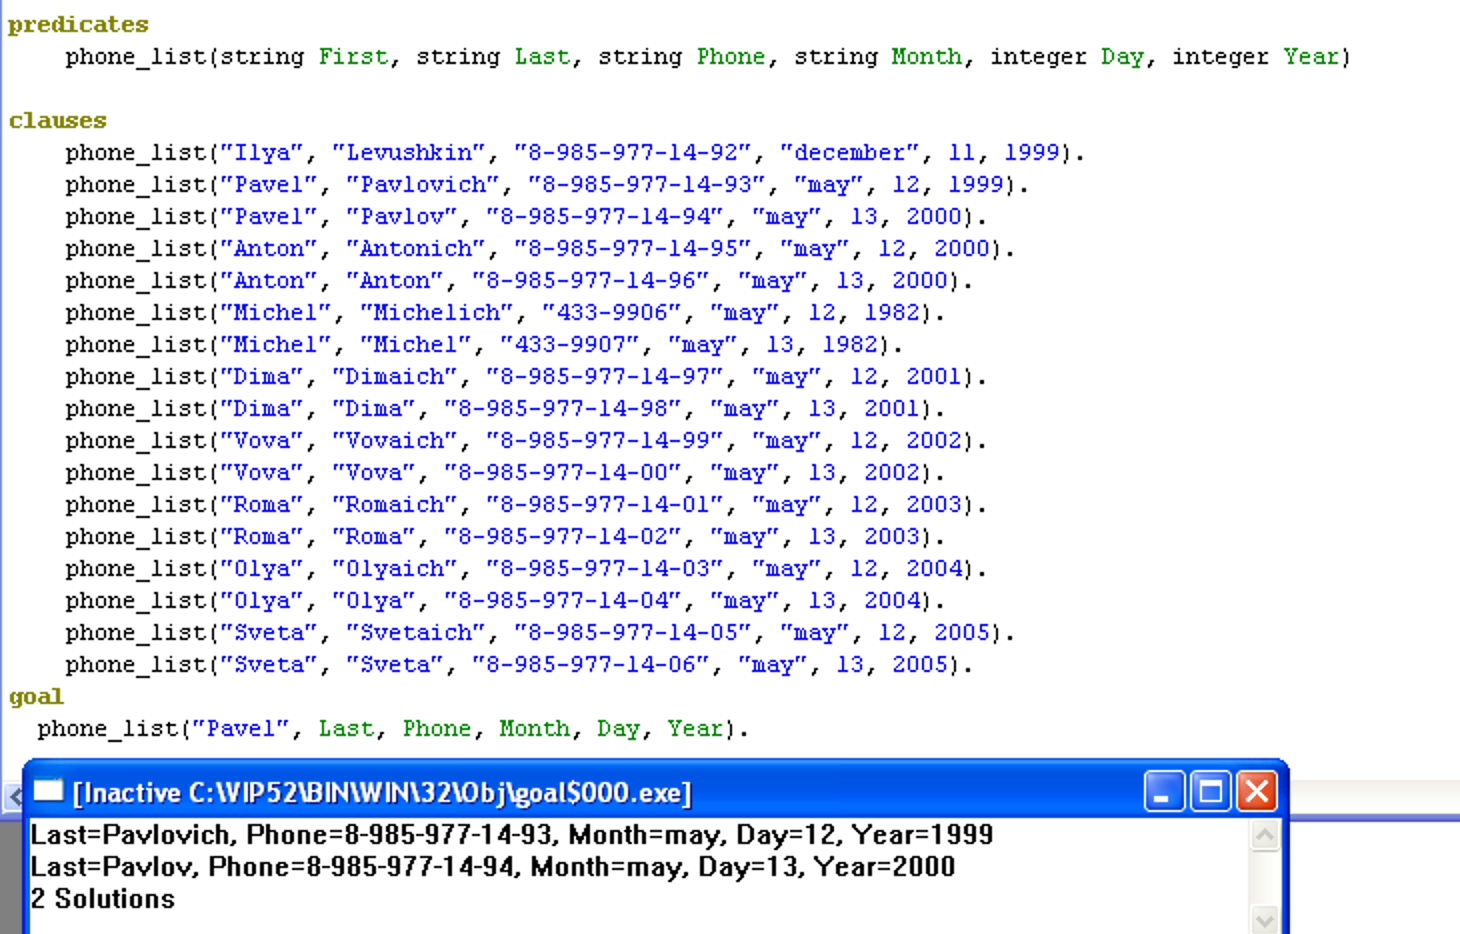
\includegraphics[scale = 0.7]{program_2.png}}
			\label{prog_2}
		\end{center}
		\caption{Программа Test.pro.}
	\end{figure}
	
	В разделе goal задается вопрос: Есть ли \textit{Pavel} в телефонной книге?
	
	Ответ будет содержать всех таких \textit{Pavel} (в данном случае двоих).

	\newpage
	
	\begin{figure}[h!]
		\begin{center}
			{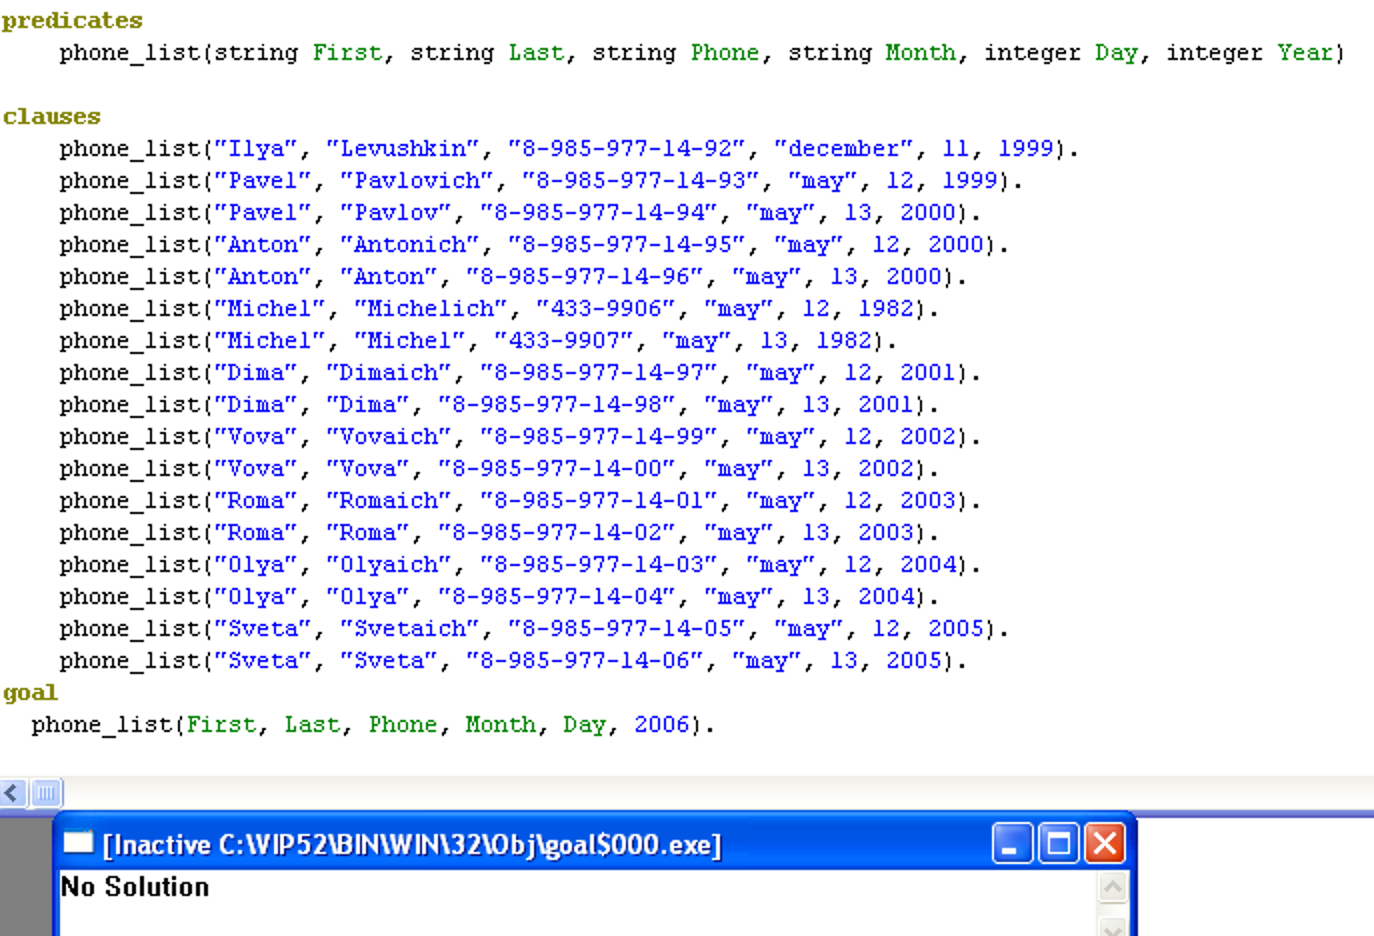
\includegraphics[scale = 0.7]{program_3.png}}
			\label{prog_3}
		\end{center}
		\caption{Программа Test.pro.}
	\end{figure}

	
	В разделе goal задается вопрос: Есть ли кто-то \textit{2006}-ого года рождения в телефонной книге?
	
	Ответ будет содержать всех таких людей, кто родился в \textit{2006} году (в данном случае ни одного).
	
	\section{Ответы на вопросы}
	
	\subsection{Что собой представляет программа на Prolog?}
	
	Программа на Prolog представляет собой базу знаний и вопрос.
	
	\begin{itemize}
		\item База знаний состоит из предложений - CLAUSES (отдельных знаний или утверждений): фактов и правил.
	
		\item Вопрос состоит только из тела – составного терма (или нескольких составных термов). Вопросы используются для выяснения выполнимости некоторого отношения между описанными в программе объектами. Система рассматривает вопрос как цель, к которой (к истинности которой) надо стремиться.
	\end{itemize}
	
	\subsection{Какова структура программы на Prolog?}
	
		\begin{itemize}
		\item База знаний состоит из предложений - CLAUSES (отдельных знаний или утверждений): фактов и правил.
		
		\item Вопрос состоит только из тела – составного терма (или нескольких составных термов). Вопросы используются для выяснения выполнимости некоторого отношения между описанными в программе объектами. Система рассматривает вопрос как цель, к которой (к истинности которой) надо стремиться.
	\end{itemize}
	
	\subsection{Как она реализуется на Prolog?}
	
	\begin{itemize}
		\item Предложения бывают двух видов: факты и правила;
		\item Каждое предложение заканчивается точкой;
		\item Предложение более общего вида – правило имеет вид:
$A :- B1,... , Bn$
		
		A называется заголовком правила, а B1,..., Bn – телом правила;
		\item Факт – это предложение, в котором отсутствует тело (частный случай правила);
	\end{itemize}
	
	
	\subsection{Как формируются результаты работы программы?}
	
	Ответ на поставленный вопрос система дает в логической форме – «Да» или «нет». Цель системы состоит в том, чтобы на поставленный вопрос найти возможность, исходя из базы знаний, ответить «Да». Вариантов ответить «Да» на поставленный вопрос может быть несколько. Система может (в нашем случае обучения - должна) быть  настроена в режим получения всех возможных вариантов ответа «Да» на поставленный вопрос.
	
	Поиск содержательного ответа на поставленный вопрос, с помощью имеющейся базы знаний, фактически заключается в поиске нужного знания, но какое знание понадобится – заранее неизвестно. Этот поиск осуществляется формально с помощью механизма \textit{унификации}, встроенного в систему и не доступного программисту. 
	
\end{document}